\documentclass[20pt, portrait, a0paper]{tikzposter}

% Packages
\usepackage{amsmath}
\usepackage{amssymb}
\usepackage{graphicx}
\usepackage{multicol}
\usepackage{enumitem}
\usepackage{amssymb}
\usepackage{fontspec}
\usepackage{algorithm}
\usepackage{algorithmicx}
\usepackage{algpseudocode}

\definecolor{red}{HTML}{8A3F3A}
\definecolor{yellow}{HTML}{E0BB3C}
\definecolor{blue}{HTML}{4569E0}
\definecolor{green}{HTML}{17E561}
\definecolor{other}{HTML}{6A939E}

% DTU Colors
\definecolor{dtu-corporate-red}{HTML}{990000}
\definecolor{dtu-white}{HTML}{ffffff}
\definecolor{dtu-black}{HTML}{000000}
\definecolor{dtu-blue}{HTML}{2F3EEA}
\definecolor{dtu-bright-green}{HTML}{1FD082}
\definecolor{dtu-navy-blue}{HTML}{030F4F}
\definecolor{dtu-yellow}{HTML}{F6D04D}
\definecolor{dtu-orange}{HTML}{FC7634}
\definecolor{dtu-pink}{HTML}{F7BBB1}
\definecolor{dtu-grey}{HTML}{DADADA}
\definecolor{dtu-red}{HTML}{E83F48}
\definecolor{dtu-green}{HTML}{008835}
\definecolor{dtu-purple}{HTML}{79238E}

% Set the main document font to Arial
\setmainfont{FiraCode Nerd Font}
% Title, Author, Institute
\title{\textbf{Multi-model Maintenance Scheduling}}
\author{\textbf{Christian Brunbjerg Jespersen}}
\institute{\textbf{Technical University of Denmark}}

\definecolor{maincolor}{cmyk}{0, 91, 72, 23} % A shade of blue
\definecolor{dtu}{RGB}{255, 102, 0} % A shade of orange
\tikzposterlatexaffectionproofoff
% Background
\colorlet{backgroundcolor}{dtu-grey}
\colorlet{framecolor}{black}

% Title
\colorlet{titlefgcolor}{white}
\colorlet{titlebgcolor}{dtu-navy-blue}

% Block
\colorlet{blockbodycolor}{dtu-navy-blue}
\colorlet{blocktitlecolor}{dtu-navy-blue}
\colorlet{blocktitlebgcolor}{dtu-navy-blue}
\colorlet{blocktitlefgcolor}{dtu-white}

% Innerblock
\colorlet{innerblocktitlebgcolor}{dtu-orange}
\colorlet{innerblocktitlefgcolor}{white}
\colorlet{innerblockbodybgcolor}{white}
\colorlet{innerblockbodyfgcolor}{black}

% Theme and color style
% \usetheme{Basic}
% \usecolorstyle{Default}

% Sets
\newcommand{\SetWorkOrder}[1]{W(\VarMetaTime#1)}
\newcommand{\ElementWorkOrder}{w}
\newcommand{\SetPeriod}{P(\VarMetaTime)}
\newcommand{\ElementPeriod}{p}

\newcommand{\SetResource}{R(\VarMetaTime)}
\newcommand{\ElementResource}{r}
\newcommand{\SetOperation}[2]{O_{#1}(\VarMetaTime, #2)}
\newcommand{\ElementOperation}{o}

\newcommand{\SetDays}[1]{D_{#1}(\VarMetaTime)}
\newcommand{\ElementDays}{d}
\newcommand{\SetActivity}[2]{A_{#2}(\VarMetaTime, #1)}
\newcommand{\ElementActivity}{a}

\newcommand{\SetWorkSegment}{K(\VarSupervisorAssignment{}{})}
\newcommand{\ElementWorkSegment}{k}
\newcommand{\SetTimeInstance}{I(\VarMetaTime)}
\newcommand{\ElementTimeInstance}{i}

\newcommand{\SetEvent}{E(\VarMetaTime)}
\newcommand{\ElementEvent}{e}

\newcommand{\SetScheduler}{S}
\newcommand{\ElementScheduler}{s}
\newcommand{\SetSupervisor}{Z}
\newcommand{\ElementSupervisor}{z}

\newcommand{\SetTechnician}{T(\VarMetaTime)}
\newcommand{\ElementTechnician}{t}

% Parameters
\newcommand{\ParStrategicValue}{strategic\_value_{\ElementWorkOrder \ElementPeriod}(\VarMetaTime)}
\newcommand{\ParStrategicPenalty}{strategic\_penalty}
\newcommand{\ParClusteringValue}{clustering\_value_{\ElementWorkOrder1, \ElementWorkOrder2}}
\newcommand{\ParStrategicResource}{resource_{\ElementPeriod\ElementResource}(\VarMetaTime)}

\newcommand{\ParStrategicWorkOrderWeight}{work\_order\_work_{\ElementWorkOrder \ElementResource}}
\newcommand{\ParStrategicInclude}{include(\VarMetaTime)}
\newcommand{\ParStrategicExclude}{exclude(\VarMetaTime)}
\newcommand{\ParTacticalValue}{tactical\_value_{\ElementDays\ElementOperation}(\VarMetaTime)}

\newcommand{\ParTacticalPenalty}{tactical\_penalty}
\newcommand{\ParOperationWork}[1]{work_{#1}(\VarMetaTime)}
\newcommand{\ParTacticalResource}{tactical\_resource_{\ElementDays\ElementResource}(\VarMetaTime)}
\newcommand{\ParStartStart}{start\_start_{\ElementOperation1, \ElementOperation2}}

\newcommand{\ParFinishStart}{finish\_start_{\ElementOperation1, \ElementOperation2}}
\newcommand{\ParEarliestStart}{earliest\_start_{\ElementOperation}(\VarMetaTime)}
\newcommand{\ParLatestFinish}{latest\_finish_{\ElementOperation}(\VarMetaTime)}
\newcommand{\ParNumberOfPeople}{number_{\ElementOperation}(\VarMetaTime)}

\newcommand{\ParOperatingTime}{operating\_time_{\ElementOperation}}
\newcommand{\ParDuration}{duration_{\ElementOperation}(\VarMetaTime)}
\newcommand{\ParSupervisorValue}{supervisor\_value_{\ElementActivity \ElementTechnician}(\VarMetaTime, \VarStartOfSegment{t}{}, \VarFinishOfSegment{t}{})} 
\newcommand{\ParFeasible}{feasible_{at}(\VarIncludeActivity{})}
\newcommand{\ParOperationsForWorkOrder}{work\_order\_to\_operations_{\ElementWorkOrder }}

\newcommand{\ParOperationsInWorkOrder}{operations\_in\_work\_order_{\ElementWorkOrder }}
\newcommand{\ParActivitiesForOperation}{activities\_for\_operation_{\ElementOperation}}
\newcommand{\ParLowerActivityWork}{lower\_activity\_work_{\ElementActivity}(\VarMetaTime)}
\newcommand{\ParActivityWork}[1]{activity\_work_{\ElementActivity}(\VarMetaTime, \VarActivityWork{#1})}

\newcommand{\ParPreparation}{preparation_{\ElementActivity1, \ElementActivity2}}
\newcommand{\ParEvent}{event_{\ElementTimeInstance \ElementEvent}}
\newcommand{\ParEventDuration}{duration_{\ElementTimeInstance \ElementEvent}}
\newcommand{\ParConstraintLimit}{constraint\_limit}

\newcommand{\ParTimeWindowStart}{time\_window\_start_{\ElementActivity}(\VarTacticalWork{}{})}
\newcommand{\ParTimeWindowFinish}{time\_window\_finish_{\ElementActivity}(\VarTacticalWork{}{})}
\newcommand{\ParAvailabilityStart}{availability\_start(\VarMetaTime)}
\newcommand{\ParAvailabilityFinish}{availability\_finish(\VarMetaTime)}

% Variables
\newcommand{\VarStrategicWorkOrderAssignment}[2]{\alpha_{#1#2}(\VarMetaTime)}
\newcommand{\VarStrategicExcess}{\epsilon_{\ElementPeriod\ElementResource}(\VarMetaTime)}
\newcommand{\VarTacticalWork}[2]{\beta_{#1#2}(\VarMetaTime)}
\newcommand{\VarTacticalExcess}{\mu_{\ElementResource \ElementDays}(\VarMetaTime)} 

\newcommand{\VarTacticalWorkBinary}[2]{\sigma_{#1#2}(\VarMetaTime)}
\newcommand{\VarTacticalWorkBinaryConsecutive}{\eta_{\ElementDays\ElementOperation}(\VarMetaTime)}
\newcommand{\VarTacticalOperationDifference}{\Delta_{\ElementOperation}(\VarMetaTime)}
\newcommand{\VarSupervisorAssignment}[2]{\gamma_{#1#2}(\VarMetaTime)}

\newcommand{\VarSupervisorAssignmentWhole}{\phi_{\ElementOperation}(\VarMetaTime)}
\newcommand{\VarActivityWork}[1]{\rho_{#1}(\VarMetaTime)}
\newcommand{\VarProcessingTime}{\delta_{\ElementActivity\ElementWorkSegment}(\VarMetaTime)} 
\newcommand{\VarActiveSegment}[2]{\pi_{#1#2}(\VarMetaTime)}

\newcommand{\VarStartOfSegment}[2]{\lambda_{#1#2}(\VarMetaTime)}
\newcommand{\VarFinishOfSegment}[2]{\Lambda_{#1#2}(\VarMetaTime)}
\newcommand{\VarSegmentInRelation}{\omega_{\ElementActivity\ElementWorkSegment\ElementTimeInstance \ElementEvent}(\VarMetaTime)}
\newcommand{\VarIncludeActivity}[1]{\theta_{#1}(\VarMetaTime)}

% Meta variables
\newcommand{\VarMetaTime}{\tau}


\begin{document}
% Create header
% \begin{tikzpicture}[remember picture,overlay]
%     % \node[fill=maincolor, minimum width=\paperwidth, minimum height=10cm, text=white] (header) at (current page.north) {
%     %     \begin{minipage}{0.9\paperwidth}
%     %         % \centering
%     %         % \vspace{1cm}
%     %         % \huge \textbf{\@title} \\[0.5cm]
%     %         % \Large \textit{\@author} - \@institute
%     %         % \vspace{1cm}
%     %     \end{minipage}
%     % };
% \end{tikzpicture}
% Title block
% \block{Header Block}{Header}
% \begin{tikzpicture}[remember picture,overlay]
    % \node[fill=maincolor, minimum width=\paperwidth, minimum height=10cm, text=white] at (current page.north) {
    %     \begin{minipage}{0.9\paperwidth}
    %         \centering
    %         \vspace{1cm}
    %         \scalebox{1.5}{\Huge \textbf{\textsf{\@title}}} \\[0.5cm]  % Larger, bold, sans-serif title
    %         \Large \textit{\@author} \\
    %         \Large \textit{\@institute}
    %         \vspace{1cm}
    %     \end{minipage}
    % };
% \end{tikzpicture}
\maketitle[innersep=4cm, width=\textwidth, roundedcorners=0.2cm, titletotopverticalspace=0, titletoblockverticalspace=2cm]

% Start of poster content
\begin{columns}

% Column 1
\column{0.60}

\block[titleinnersep=0.5cm, roundedcorners=0.2cm, titleleft]{Introduction}{
	Current Operation Research methods have proven difficult to implement in operational settings. The poster
	presents a methodology to decompose a large-scale decision process into a series of modules that each represents
	the decisions taken by each individual stakeholder making up the scheduling process. 
}

\block[titleinnersep=0.5cm, roundedcorners=0.2cm, titleleft]{Research Questions}{
	
  \begin{enumerate}[label=\arabic*.]
    \item How to implement a scheduling system that can coordinate in real-time?
	\item How to coordinate multiple stakeholders in real-time that has different mathematical model requirements?
	\item How to synchronize state across a high number of metaheuristics spread across different CPU threads?
	\item How to intergrate metaheuristics into the workflow of a working scheduler?
    \item Can you coordinate metaheuristics based on different mathematical models in real-time?
	\item Which modern software architecture should be used to create scalabily metaheuristic based scheduling systems
	\item Which of the latest techniques in modern software development can be utilized to integrate metaheuristics directly into a business' IT infrastructure
	\item How to create modular algorithm components that can solve well defined decision problems while also integrating into a larger decision making process
	\item 
  \end{enumerate}

}

\block[titleinnersep=0.5cm, bodyverticalshift=0cm, roundedcorners=0.2cm, titleleft]{Solution Method}{
	\innerblock[roundedcorners=0.2cm, bodyinnersep=1.0cm]{Modular Scheduling System Architecture}{
	\usetikzlibrary {positioning}

\definecolor{red}{HTML}{8A3F3A}
\definecolor{yellow}{HTML}{E0BB3C}
\definecolor{blue}{HTML}{4569E0}
\definecolor{green}{HTML}{17E561}
\definecolor{other}{HTML}{6A939E}

% DTU Colors
\definecolor{dtu-corporate-red}{HTML}{990000}
\definecolor{dtu-white}{HTML}{ffffff}
\definecolor{dtu-black}{HTML}{000000}
\definecolor{dtu-blue}{HTML}{2F3EEA}
\definecolor{dtu-bright-green}{HTML}{1FD082}
\definecolor{dtu-navy-blue}{HTML}{030F4F}
\definecolor{dtu-yellow}{HTML}{F6D04D}
\definecolor{dtu-orange}{HTML}{FC7634}
\definecolor{dtu-pink}{HTML}{F7BBB1}
\definecolor{dtu-grey}{HTML}{DADADA}
\definecolor{dtu-red}{HTML}{E83F48}
\definecolor{dtu-green}{HTML}{008835}
\definecolor{dtu-purple}{HTML}{79238E}


\newcommand{\ModelColor}{dtu-red}
\newcommand{\UserInterfaceColor}{dtu-yellow}
\newcommand{\PersistenceColor}{dtu-blue}
\newcommand{\PointerSwapColor}{dtu-green}
\newcommand{\OrchestratorColor}{dtu-bright-green}

\newcommand{\basisinput}{4cm}  % Default value if not set by /graph/basis

\pgfkeys{
	/graph/.is family, /graph,
	default/.style = {
		show_shared_pointer = false,
		show_orchestrator = false,
		show_persistence = false,
		show_user_interface = false,
		basisinput/.estore in = \basisinput,
	},
	show_shared_pointer/.estore in = \ShowSharedSolutionCommunication,
	show_orchestrator/.estore in = \ShowOrchestratorCommunication,
	show_persistence/.estore in = \ShowPersistenceCommunication,
	show_user_interface/.estore in = \ShowUserInterfaceCommunication,
	basisinput/.estore in = \basisinput,
}

\newlength{\basis}
\tikzset{
  basis/.code={\setlength{\basis}{\basisinput}}, % TikZ assignment code
  basis/.default=3cm,                   % Provide a default (\b@sis is undefined/unassigned)
  basis,                                % Set initial Value (\b@sis is defined/assigned)
}

\newcommand{\drawOrdinatorArchitecture}[1]{
	\pgfkeys{/graph, default, #1}
	\setlength{\basis}{\basisinput}
	\begin{tikzpicture}[scale=0.75, line width=0.05\basis]

		\ifthenelse{\equal{\ShowOrchestratorCommunication}{true}}{
			\draw[color=other,-, ultra thick] (Strategic) -- (Orchestrator);
			\draw[color=other,-, ultra thick] (Tactical) -- (Orchestrator);
			\draw[color=other,-, ultra thick] (Supervisor) -- (Orchestrator);
			\draw[color=other,-, ultra thick] (Operational_1) -- (Orchestrator);
			\draw[color=other,-, ultra thick] (Operational_2) -- (Orchestrator);
			\draw[color=other,-, ultra thick] (Operational_3) -- (Orchestrator);
		}{}
		% \draw[help lines] (0\basis, 0\basis) grid (10\basis, 8\basis);
		\draw (5\basis,4\basis) node[minimum height=5\basis,minimum width=7.0\basis,rounded corners=0.1\basis] {};

	    \draw[draw=black] (4.125\basis,4.0\basis) node[opacity=0.5, minimum height=3.5\basis,minimum width=6.25\basis,rounded corners=0.1\basis,fill=\PointerSwapColor] {} ;
	    \draw (2.5\basis,5.5\basis) node[minimum height=1\basis,minimum width=1\basis,fill=\ModelColor,rounded corners=0.1\basis] (Strategic) {Stra};
	    \draw (5.0\basis,4.0\basis) node[minimum height=1\basis,minimum width=1\basis,fill=\ModelColor,rounded corners=0.1\basis] (Supervisor) {Sup};
		\draw (7.5\basis,5.5\basis) node[minimum height=1\basis,minimum width=1\basis,fill=\ModelColor,rounded corners=0.1\basis] (Tactical) {Tac};

		\draw (2.5\basis,2.5\basis) node[minimum height=1\basis,minimum width=1\basis,fill=\ModelColor,rounded corners=0.1\basis] (Operational_1) {$O_{1}$};
		\draw (5.0\basis,2.5\basis) node[minimum height=1\basis,minimum width=1\basis,fill=\ModelColor,rounded corners=0.1\basis] (Operational_2) {$O_{2}$};
		\draw (7.5\basis,2.5\basis) node[minimum height=1\basis,minimum width=1\basis,fill=\ModelColor,rounded corners=0.1\basis,rounded corners=0.1\basis] (Operational_3) {$O_{3}$};
	
		\draw (Strategic) edge (Tactical);
		\draw (Strategic) edge (Tactical);
		\draw (5\basis,5.5\basis) edge (Supervisor);
		\draw (Supervisor) -- (2.5\basis,4.0\basis) -- (Operational_1);
		\draw (Supervisor) edge (Operational_2);
		\draw (Supervisor) -- (7.5\basis,4.0\basis) -- (Operational_3);
		\draw (5.0\basis,0.5\basis)   node[minimum height=1\basis,minimum width=5.0\basis,                fill=\PersistenceColor,rounded corners=0.1\basis] {persistence};
		\draw (5.0\basis,7.5\basis)   node[minimum height=1\basis,minimum width=5.0\basis,                fill=\OrchestratorColor,rounded corners=0.1\basis] (Orchestrator) {Orchestrator};
		\draw (0.5\basis,4.0\basis)   node[rotate=90, minimum height=1.0\basis, minimum width=3.5\basis,  fill=\PointerSwapColor,rounded corners=0.1\basis] {decision variables};
		\draw (9.5\basis,5.75\basis)  node[rotate=90, minimum height=1.0\basis, minimum width=1.0\basis,  fill=\UserInterfaceColor,rounded corners=0.1\basis] {UI};
		\draw (9.5\basis,4.0\basis)   node[rotate=90, minimum height=1.0\basis, minimum width=1.0\basis,  fill=\UserInterfaceColor,rounded corners=0.1\basis] {UI};
		\draw (9.5\basis,2.25\basis)  node[rotate=90, minimum height=1.0\basis, minimum width=1.0\basis,  fill=\UserInterfaceColor,rounded corners=0.1\basis] {UI};

		% Legend
		\begin{scope}[shift={(11.0\basis,5.7\basis)}]
			\node at (-0.25\basis,1\basis) [right] {};
			\draw[color=\OrchestratorColor,fill,rounded corners=0.1\basis] (0\basis,0.0\basis)   rectangle (0.5\basis, 0.5\basis);
			\node[anchor=west] at (0.5\basis, 0.25\basis) { Managing metaheuristic lifetimes };
			\draw[color=\PointerSwapColor,fill,rounded corners=0.1\basis] (0\basis,-1.0\basis)   rectangle(0.5\basis, -0.5\basis); 
			\node[anchor=west] at (0.5\basis, -0.75\basis) { Solution sharing (Atomic pointer swaps) };
			\draw[color=\ModelColor,fill,rounded corners=0.1\basis] (0\basis,-2.0\basis)         rectangle(0.5\basis, -1.5\basis); 
			\node[anchor=west] at (0.5\basis, -1.75\basis) { Metaheurics (Mathematical Models) };
			\draw[color=\PersistenceColor,fill,rounded corners=0.1\basis] (0\basis,-3.0\basis)   rectangle(0.5\basis, -2.5\basis); 
			\node[anchor=west] at (0.5\basis, -2.75\basis) { Data storage (Memory locks)};
			\draw[color=\UserInterfaceColor,fill,rounded corners=0.1\basis] (0\basis,-4.0\basis) rectangle(0.5\basis, -3.5\basis); 
			\node[anchor=west] at (0.5\basis, -3.75\basis) { Message passing (Memory channels) };

		\end{scope}
		\ifthenelse{\equal{\ShowSharedSolutionCommunication}{true}}{
			\draw[->, thick] (Strategic) -- (Orchestrator);
		}{}
		\ifthenelse{\equal{\ShowUserInterfaceCommunication}{true}}{
			\draw[->, thick] (Strategic) -- (Orchestrator);
		}{}
		\ifthenelse{\equal{\ShowPersistenceCommunication}{true}}{
			\draw[->, thick] (Strategic) -- (Orchestrator);
		}{}
		

	\end{tikzpicture}
}


	\drawGraph{basisinput=3cm}
	}
}
\begin{subcolumns}

\subcolumn{0.5} \block[titleinnersep=0.5cm, roundedcorners=0.2cm, titleleft, bodyinnersep=0.5cm]{Algorithm: Actor based Large Neighborhood Search}{
	\scalebox{0.9}{
		\begin{minipage}{0.27\textwidth}
			\newcommand{\MessageQueue}{Q}
\newcommand{\Solution}{X}
\newcommand{\ProblemInstance}{P}
\newcommand{\SharedSolution}{S}

\begin{algorithm}[H]
\caption{Actor-based Large Neighborhood Search} 
\begin{algorithmic}[1]
\State \textbf{Input} $\MessageQueue$    = message queue
\State \textbf{Input} $\ProblemInstance$ = problem instance
\State \textbf{Input} $\Solution$        = initial schedule
\State \textbf{Input} $\SharedSolution$  = shared solution
% \State $\Solution^b = \Solution$
\Repeat \label{alg:actor-based-large-neighborhood-search:main-optimization-loop}
	\State $\Solution^t = clone(\Solution)$ \label{alg:actor-based-large-neighborhood-search:clone-solution}
	\While{$\MessageQueue.has\_message()$} \label{alg:actor-based-large-neighborhood-search:message-loop}
        % \State $m = queue.pop()$
        % \State $m.destruct(\Solution^b)$
		\State $\ProblemInstance.update(\SharedSolution, m)$
        \State $\Solution^t.destruct(\SharedSolution, m)$
    \EndWhile
	
    \State $\Solution^t.repair(\SharedSolution)$ \label{alg:actor-based-large-neighborhood-search:repair}

    \If{accept($\Solution^t, \Solution$)} \label{alg:actor-based-large-neighborhood-search:accept}                       
        \State $\Solution.update(\Solution^t)$
    \EndIf                                         

    \If{$c(\Solution^t) < c(\Solution)$} \label{alg:actor-based-large-neighborhood-search:better-solution}                             
        \State $\Solution.update(\Solution^t)$
		\State $\SharedSolution.atomic\_pointer\_swap(\Solution)$
    \EndIf                                           
	\State $\MessageQueue.push(m)$ \label{alg:actor-based-large-neighborhood-search:schedule-message}
\Until
\end{algorithmic}
\label{alg:actor-based-large-neighborhood-search}
\end{algorithm}


		\end{minipage}
	}
}
\block[titleinnersep=0.5cm, roundedcorners=0.2cm, titleleft]{Results}{
  \begin{itemize}
    \item \textbf{Improved Efficiency}: Achieved a 15\% reduction in total costs across the supply chain.
    \item \textbf{Stakeholder Satisfaction}: Increased satisfaction scores among all actors by 20\%.
    \item \textbf{Collaborative Strategies}: Developed joint policies that benefit all parties.
  \end{itemize}
}

\subcolumn{0.5} 
\block[titleinnersep=0.5cm, roundedcorners=0.2cm, titleleft]{Future Work}{
  \begin{itemize}
    \item Extend the approach to international supply chains.
    \item Incorporate real-time data analytics for dynamic decision-making.
    \item Explore applications in other sectors like healthcare and transportation.
  \end{itemize}
}

\block[titleinnersep=0.5cm, roundedcorners=0.2cm, titleleft]{Conclusion}{
	
}

\end{subcolumns}
% Column 2
\column{0.40}
	\blockbodyinnersep=2cm
\block[bodyinnersep=1cm, titleinnersep=0.5cm, roundedcorners=0.2cm, titleleft]{Methodology}{
  	\innerblock[roundedcorners=0.2cm]{Strategic}{
		\scalebox{0.5}{
			\begin{minipage}{0.66\textwidth}
				
\newpage
\begin{alignat}{2}
	& \text{\rule{\linewidth}{0.4pt}} \notag\\
	& \textbf{Meta variables:} \notag\\
	& \ElementScheduler \in \SetScheduler \\
	& \VarTacticalWork{}{} \\ 
	& \tau \in [0, \infty] \\
	& \text{\rule{\linewidth}{0.4pt}} \notag\\
	& \textbf{Minimize:} \notag                                                                                                                                                        \\
	& \sum_{\ElementWorkOrder \in \SetWorkOrder{}} \sum_{\ElementPeriod \in \SetPeriod} \ParStrategicValue \cdot \VarStrategicWorkOrderAssignment{\ElementWorkOrder}{\ElementPeriod}  \notag\\ 
	& + \sum_{\ElementPeriod \in \SetPeriod} \sum_{\ElementResource \in \SetResource} \ParStrategicPenalty \cdot \VarStrategicExcess     \notag                                              \\
	& + \sum_{\ElementPeriod \in \SetPeriod} \sum_{\ElementWorkOrder1 \in \SetWorkOrder{}} \sum_{\ElementWorkOrder2 \in \SetWorkOrder{}} 	 \quad \ParClusteringValue \cdot \VarStrategicWorkOrderAssignment{\ElementWorkOrder1}{\ElementPeriod} \cdot \VarStrategicWorkOrderAssignment{\ElementWorkOrder2}{\ElementPeriod}  \\
	& \text{\rule{\linewidth}{0.4pt}} \notag\\
	& \textbf{Subject to:} \notag                                                                                                                                                      \\
	& \sum_{\ElementWorkOrder \in \SetWorkOrder{}} \ParStrategicWorkOrderWeight \cdot \VarStrategicWorkOrderAssignment{\ElementWorkOrder}{\ElementPeriod} \leq \ \ParStrategicResource + \VarStrategicExcess                                                                           \quad \forall \ElementPeriod \in \SetPeriod \quad \forall \ElementResource \in \SetResource                                                                                      \\
	& \sum_{\ElementWorkOrder \in \SetWorkOrder{}} \VarStrategicWorkOrderAssignment{\ElementWorkOrder}{\ElementPeriod} = 1              \quad \forall \ElementPeriod \in \SetPeriod                                                                                                                                      \\
	& \VarStrategicWorkOrderAssignment{\ElementWorkOrder}{\ElementPeriod} = 0                                                            \quad \forall (\ElementWorkOrder, \ElementPeriod) \in \ParStrategicExclude                                                                                                       \\
	& \VarStrategicWorkOrderAssignment{\ElementWorkOrder}{\ElementPeriod} = 1                                                            \quad \forall (\ElementWorkOrder, \ElementPeriod) \in \ParStrategicInclude                                                                                                       \\
	& \VarStrategicWorkOrderAssignment{\ElementWorkOrder}{\ElementPeriod} \in \{0, 1\}                                                   \quad \forall \ElementWorkOrder \in \SetWorkOrder{} \quad \forall \ElementPeriod \in \SetPeriod                                                                                 \\ 
	& \VarStrategicExcess \in \mathbb{R}^{+}                                                                                             \quad \forall \ElementPeriod \in \SetPeriod \quad \forall \ElementResource \in \SetResource                                                                                  \\ 
	& \text{\rule{\linewidth}{0.4pt}} \notag
\end{alignat}
\newpage


			\end{minipage}
		}
	}
	\vspace{1cm}
	\innerblock[roundedcorners=0.2cm]{Tactical}{
		\scalebox{0.5}{
			\begin{minipage}{0.66\textwidth}
				\section{The Tactical Model}
\begin{itemize}
	\item Respect precedence constraints
	\item Respect daily resource requirements for each trait
	\item Penalize exceeded daily capacity
\end{itemize}

After the strategic model has optimized its schedule the tactical agent will continue scheduling the output at a more detailed level. This means that now the tactical agent will schedule 
out on each of the days of the work orders scheduled by the strategic agent. 

The tactical model is responsible for providing an initial suggestion for a weekly schedule, below we see the model for the tactical agent.
\begin{alignat}{2}
	& \textbf{Meta variables:} \notag\\
	& \ElementScheduler = \SetScheduler \notag\\
	& \tau \in [0, \infty] \notag\\
	& \VarStrategicWorkOrderAssignment{}{} \notag\\
	& \textbf{Minimize:} \notag\\
	& \sum_{\ElementOperation \in \SetOperation{}{\VarStrategicWorkOrderAssignment{}{}}} \sum_{\ElementDays \in \SetDays{}} \ParTacticalValue!!!!!!!!!!!!! \cdot \VarTacticalWork{\ElementDays}{\ElementOperation}\notag\\  
	& + \sum_{r \in \SetResource} \sum_{\ElementDays \in \SetDays{}} \ParTacticalPenalty \cdot \VarTacticalExcess                                               \\  
	& \textbf{Subject to:}                                                          \notag                                                                   \\
	& \sum_{\ElementOperation \in \SetOperation{}{\VarStrategicWorkOrderAssignment{}{}}} \ParOperationWork{\ElementOperation} \cdot \VarTacticalWork{\ElementDays}{\ElementOperation}\notag\\
	& \quad \leq \ParTacticalResource + \VarTacticalExcess\notag\\ 
	& \quad \forall \ElementDays \in \SetDays{} \quad \forall r \in \SetResource\\ 
	& \sum_{\ElementDays = \ParEarliestStart}^{\ParLatestFinish} \VarTacticalWorkBinary{\ElementDays}{\ElementOperation} = \ParDuration \notag\\
	& \quad \forall \ElementOperation \in \SetOperation{}{\VarStrategicWorkOrderAssignment{}{}} \\
	& \sum_{\ElementDays^* \in  \SetDays{\ParDuration}} \VarTacticalWorkBinary{\ElementDays^*}{\ElementOperation} \notag\\
	& \quad = \ParDuration \cdot \VarTacticalWorkBinaryConsecutive \notag\\ 
	& \quad \forall \ElementOperation \in \SetOperation{}{\VarStrategicWorkOrderAssignment{}{}} \quad \forall \ElementDays \in \SetDays{} \\
	& \sum_{\ElementOperation \in \SetOperation{}{\VarStrategicWorkOrderAssignment{}{}}} \VarTacticalWorkBinaryConsecutive = 1, \notag\\
	& \quad \forall \ElementDays \in \SetDays{} \notag\\
	& \sum_{\ElementDays \in \SetDays{}} \ElementDays \cdot \VarTacticalWorkBinary{\ElementDays}{\ElementOperation1} + \VarTacticalOperationDifference  = \sum_{\ElementDays \in \SetDays{}} \ElementDays \cdot \VarTacticalWorkBinary{\ElementDays}{\ElementOperation2}                   \notag  \\ 
	& \quad \forall (o1, \ElementOperation2) \in \ParFinishStart                                                           \\ 
	& \sum_{\ElementDays \in \SetDays{}} \ElementDays \cdot \VarTacticalWorkBinary{\ElementDays}{\ElementOperation1} = \sum_{\ElementDays \in \SetDays{}} \ElementDays \cdot \VarTacticalWorkBinary{\ElementDays}{\ElementOperation2}  \notag                               \\ 
	& \quad \forall (o1, \ElementOperation2) \in \ParStartStart                                                       \\ 
	& \VarTacticalWork{\ElementDays}{\ElementOperation} \leq \ParNumberOfPeople \cdot \ParOperatingTime \notag                                                     \\ 
	& \quad \forall \ElementDays \in \SetDays{} \quad \forall \ElementOperation \in \SetOperation{}{\VarStrategicWorkOrderAssignment{}{}}                                                                  \\
	& \VarTacticalWork{\ElementDays}{\ElementOperation} \in \mathbb{R} \quad \notag\\
	& \quad \forall \ElementDays \in \SetDays{} \quad \forall \ElementOperation \in \SetOperation{}{\VarStrategicWorkOrderAssignment{}{}}                                         \\
	& \VarTacticalExcess \in \mathbb{R} \quad\notag\\
	& \quad \forall r \in \SetResource \quad \forall \ElementDays \in \SetDays{}                                        \\
	& \VarTacticalWorkBinary{\ElementDays}{\ElementOperation} \in \{0, 1\}\quad \notag\\
	& \quad \forall \ElementDays \in \SetDays{} \quad \forall \ElementOperation \in \SetOperation{}{\VarStrategicWorkOrderAssignment{}{}} \\
	& \VarTacticalWorkBinaryConsecutive \in \{0, 1\}\quad \notag\\
	& \quad \forall \ElementDays \in \SetDays{} \quad \forall \ElementOperation \in \SetOperation{}{\VarStrategicWorkOrderAssignment{}{}} \\
	& \VarTacticalOperationDifference \in \{0, 1\} \\
	& \quad \forall \ElementOperation \in \SetOperation{}{\VarStrategicWorkOrderAssignment{}{}}                                      \\
	& \VarMetaTime \in  [0, \infty] 
\end{alignat}


			\end{minipage}
		}
	}
	\vspace{1cm}
	\innerblock[roundedcorners=0.2cm]{Supervisor}{
		\scalebox{0.5}{
			\begin{minipage}{0.66\textwidth}
				\section{The Supervisor Model}
The maintenance supervisor is considered the most central person in a maintenance scheduling system. 
All the work of the planner and scheduler should be considered a service for the supervisor.

The supervisor has multiple different responsibilities among them are: 

\begin{itemize}
	\item Assigning work orders
	\item Creating a daily schedule
	\item Keeping the schedule up-to-date
\end{itemize}


\begin{alignat}{2}
	& \textbf{Meta variables:} \notag\\
	& \tau \in [0, \infty] \notag\\
	& \ElementSupervisor \in \SetSupervisor \notag\\
	& \VarStrategicWorkOrderAssignment{}{} \notag\\
	& \VarIncludeActivity{} \notag\\
	& \textbf{Maximize:} \notag\\
	& \sum_{\ElementActivity \in \SetActivity{\VarStrategicWorkOrderAssignment{}{}}{}} \sum_{\ElementTechnician \in \SetTechnician} \ParSupervisorValue \cdot \VarSupervisorAssignment{\ElementActivity}{\ElementTechnician} \\ 
	& \textbf{Subject to:} \notag\\ 
	& \sum_{\ElementActivity \in \SetActivity{\VarStrategicWorkOrderAssignment{}{}}{\ElementOperation}} \VarActivityWork{\ElementActivity} = \ParOperationWork{\ElementOperation}   \notag\\
	& \quad \forall \ElementOperation \in \SetOperation{}{\VarStrategicWorkOrderAssignment{}{}}\\
	& \sum_{\ElementTechnician \in \SetTechnician} \sum_{\ElementActivity \in \SetActivity{\VarStrategicWorkOrderAssignment{}{}}{\ElementOperation}}\VarSupervisorAssignment{\ElementActivity}{\ElementTechnician} = \VarSupervisorAssignmentWhole \cdot \ParNumberOfPeople \notag\\
	& \quad \forall \ElementOperation \in \SetOperation{}{\VarStrategicWorkOrderAssignment{}{}}  \\
	& \sum_{\ElementOperation \in \SetOperation{\ElementWorkOrder}{\VarStrategicWorkOrderAssignment{}{}}} \VarSupervisorAssignmentWhole = !!!! |\SetOperation{\ElementWorkOrder}{\VarStrategicWorkOrderAssignment{}{}}| \notag\\ 
	& \quad \forall \ElementWorkOrder \in \SetWorkOrder{,\VarStrategicWorkOrderAssignment{}{}} \\
	& \sum_{\ElementActivity \in \SetActivity{\VarStrategicWorkOrderAssignment{}{}}{\ElementOperation}} \VarSupervisorAssignment{\ElementActivity}{\ElementTechnician} \leq 1 \notag\\
	& \quad \forall \ElementOperation \in \SetOperation{}{\VarStrategicWorkOrderAssignment{}{}} \quad \forall \ElementTechnician \in \SetTechnician \\  
	& \VarSupervisorAssignment{\ElementActivity}{\ElementTechnician} \leq \ParFeasible \notag\\
	& \quad \forall \ElementOperation \in \SetOperation{}{\VarStrategicWorkOrderAssignment{}{}} \quad \forall \ElementTechnician \in \SetTechnician \\
	& \VarSupervisorAssignment{\ElementActivity}{\ElementTechnician} \in \{0, 1\} \notag\\
	& \quad \forall \ElementOperation \in \SetOperation{}{\VarStrategicWorkOrderAssignment{}{}} \quad \forall \ElementTechnician \in \SetTechnician \\ 
	& \VarActivityWork{\ElementActivity} \in [\ParLowerActivityWork, \ParOperationWork{\ElementActivity}] \notag\\
	& \quad \forall \ElementActivity \in \SetActivity{\VarStrategicWorkOrderAssignment{}{}}{} \\
    & \VarMetaTime \in  [0, \infty] 
\end{alignat}

In the supervisor model shown in \ref{} the set $O$ and $W$ comes from the tactical algorithm
and value $v$ and the information of whether or not the operation can be assigned to a 
specific operational model comes from the operational model itself and is captured in the.

Can this be done? What should the Supervisor have here? He should have what is necessary to
handle the. 

			\end{minipage}
		}
	}
	\vspace{1cm}
	\innerblock[roundedcorners=0.2cm]{Operational}{
		\scalebox{0.5}{
			\begin{minipage}{0.66\textwidth}
				\begin{alignat}{2}
	& \text{\rule{\linewidth}{0.4pt}} \notag\\
	& \textbf{Meta variables:}                                                                                                                                                                         \notag\\
	& \ElementTechnician \in \SetTechnician                                                                                                                                                            \\
	& \VarStrategicWorkOrderAssignment{}{}                                                                                                                                                             \\
	& \VarSupervisorAssignment{}{}                                                                                                                                                                     \\
	& \tau \in [0, \infty]                                                                                                                                                                             \\
	& \text{\rule{\linewidth}{0.4pt}} \notag\\
	& \textbf{Maximize:}                                                                                                                                                                               \notag\\
	& \sum_{\ElementActivity \in \SetActivity{\VarSupervisorAssignment{}{\ElementTechnician}}{}} \sum_{\ElementWorkSegment \in \SetWorkSegment} \VarProcessingTime                                           \\
	& \text{\rule{\linewidth}{0.4pt}} \notag\\
	& \textbf{Subject to:}                                                                                                                                                                             \notag\\
    & \sum_{\ElementWorkSegment \in \SetWorkSegment} \VarProcessingTime \cdot \VarActiveSegment{\ElementActivity}{\ElementWorkSegment} = \ParActivityWork{} \cdot \VarIncludeActivity{\ElementActivity}                                                                                                                                            \quad \forall \ElementActivity \in \SetActivity{\VarSupervisorAssignment{}{\ElementTechnician}}{}                                                                                                      \\
	& \VarStartOfSegment{\ElementActivity2}{1} \geq \VarFinishOfSegment{\ElementActivity1}{last(\ElementActivity1)} + \ParPreparation                                                                    \quad \forall \ElementActivity1 \in \SetActivity{\VarSupervisorAssignment{}{\ElementTechnician}}{} \quad \forall \ElementActivity2 \in \SetActivity{\VarSupervisorAssignment{}{\ElementTechnician}}{}  \\
	& \VarStartOfSegment{\ElementActivity}{\ElementWorkSegment} \geq \VarFinishOfSegment{\ElementActivity}{\ElementWorkSegment-1} - \ParConstraintLimit \cdot (2 - \VarActiveSegment{\ElementActivity}{\ElementWorkSegment} + \VarActiveSegment{\ElementActivity}{\ElementWorkSegment-1})                                                                      \notag\\
	& \quad \forall \ElementActivity \in \SetActivity{\VarSupervisorAssignment{}{\ElementTechnician}}{} \quad\forall \ElementWorkSegment \in \SetWorkSegment                                                 \\ 
	& \VarProcessingTime = \VarFinishOfSegment{\ElementActivity}{\ElementWorkSegment} - \VarStartOfSegment{\ElementActivity}{\ElementWorkSegment}                                                                                                                                              \quad \forall \ElementActivity \in \SetActivity{\VarSupervisorAssignment{}{\ElementTechnician}}{}  \quad\forall \ElementWorkSegment \in \SetWorkSegment                                                \\
	& \VarStartOfSegment{\ElementActivity}{\ElementWorkSegment} \geq \ParEvent + \ParEventDuration - \ParConstraintLimit \cdot (1 - \VarSegmentInRelation) \notag\\ 
	& \quad \forall \ElementActivity \in \SetActivity{\VarSupervisorAssignment{}{\ElementTechnician}}{}  \quad\forall \ElementWorkSegment \in \SetWorkSegment                                           \quad \forall i \in \SetTimeInstance  \quad\forall \ElementEvent \in \SetEvent                                                                                                                         \\
	& \VarFinishOfSegment{\ElementActivity}{\ElementWorkSegment} \leq \ParEvent + \ParConstraintLimit \cdot \VarSegmentInRelation \notag\\
	& \quad \forall \ElementActivity \in \SetActivity{\VarSupervisorAssignment{}{\ElementTechnician}}{}  \quad\forall \ElementWorkSegment \in \SetWorkSegment                                         \quad \forall i \in \SetTimeInstance  \quad\forall \ElementEvent \in \SetEvent                                                                                                                         \\
	& \VarStartOfSegment{\ElementActivity}{1} \geq \ParTimeWindowStart  \quad \forall \ElementActivity \in \SetActivity{\VarSupervisorAssignment{}{\ElementTechnician}}{}                                                                                                      \\
	& \VarFinishOfSegment{\ElementActivity}{last(\ElementActivity)} \leq \ParTimeWindowFinish  \quad \forall \ElementActivity \in \SetActivity{\VarSupervisorAssignment{}{\ElementTechnician}}{}                                                                                                      \\
	& \VarActiveSegment{\ElementActivity}{\ElementWorkSegment} \in \{0, 1\}  \quad \forall \ElementActivity \in \SetActivity{\VarSupervisorAssignment{}{\ElementTechnician}}{} \quad \forall \ElementWorkSegment \in \SetWorkSegment                                                \\
	& \VarStartOfSegment{\ElementActivity}{\ElementWorkSegment} \in [\ParAvailabilityStart, \ParAvailabilityFinish]                                                                                                           \notag\\
	& \quad \forall \ElementActivity \in \SetActivity{\VarSupervisorAssignment{}{\ElementTechnician}}{} \quad \forall \ElementWorkSegment \in \SetWorkSegment                                                \\
	& \VarFinishOfSegment{\ElementActivity}{\ElementWorkSegment} \in [\ParAvailabilityStart, \ParAvailabilityFinish]                                                                                                             \notag\\
	& \quad \forall \ElementActivity \in \SetActivity{\VarSupervisorAssignment{}{\ElementTechnician}}{} \quad \forall \ElementWorkSegment \in \SetWorkSegment                                                \\
	& \VarProcessingTime \in [0, \ParOperationWork{\ElementActivity\_to\_o(\ElementActivity)} ]  \quad \forall \ElementActivity \in \SetActivity{\VarSupervisorAssignment{}{\ElementTechnician}}{} \quad \forall \ElementWorkSegment \in \SetWorkSegment                                                \\
	& \VarSegmentInRelation \in \{0 , 1\}                                                                                                                                                                                                                                                                                     \quad \forall \ElementActivity \in \SetActivity{\VarSupervisorAssignment{}{\ElementTechnician}}{} \quad \forall \ElementWorkSegment \in \SetWorkSegment  \quad \forall i \in \SetTimeInstance \quad \forall \ElementEvent \in \SetEvent                                                                                                                         \\
	& \VarIncludeActivity{\ElementActivity} \in \{0, 1\}                                                                                                                                      \quad \forall \ElementActivity \in \SetActivity{\VarSupervisorAssignment{}{\ElementTechnician}}{}                                                                                                     \\ 
	& \text{\rule{\linewidth}{0.4pt}} \notag
\end{alignat}

			\end{minipage}
		}
	}
}

% Column 3
% \column{0.50}

% % Contact Information
% \block[titleinnersep=0.5cm, roundedcorners=0.2cm, titleleft]{Contact Information}{
%   \begin{itemize}
%     \item \textbf{Email}: \href{mailto:your.email@institution.edu}{your.email@institution.edu}
%     \item \textbf{Phone}: +1 (234) 567-8901
%     \item \textbf{Website}: \href{http://www.yourwebsite.com}{www.yourwebsite.com}
%   \end{itemize}
% }

\end{columns}

\block[roundedcorners=0.2cm, bodywidthscale=1.0, bodyverticalshift=0cm]{}{
	\begin{minipage}{0.12\linewidth}
		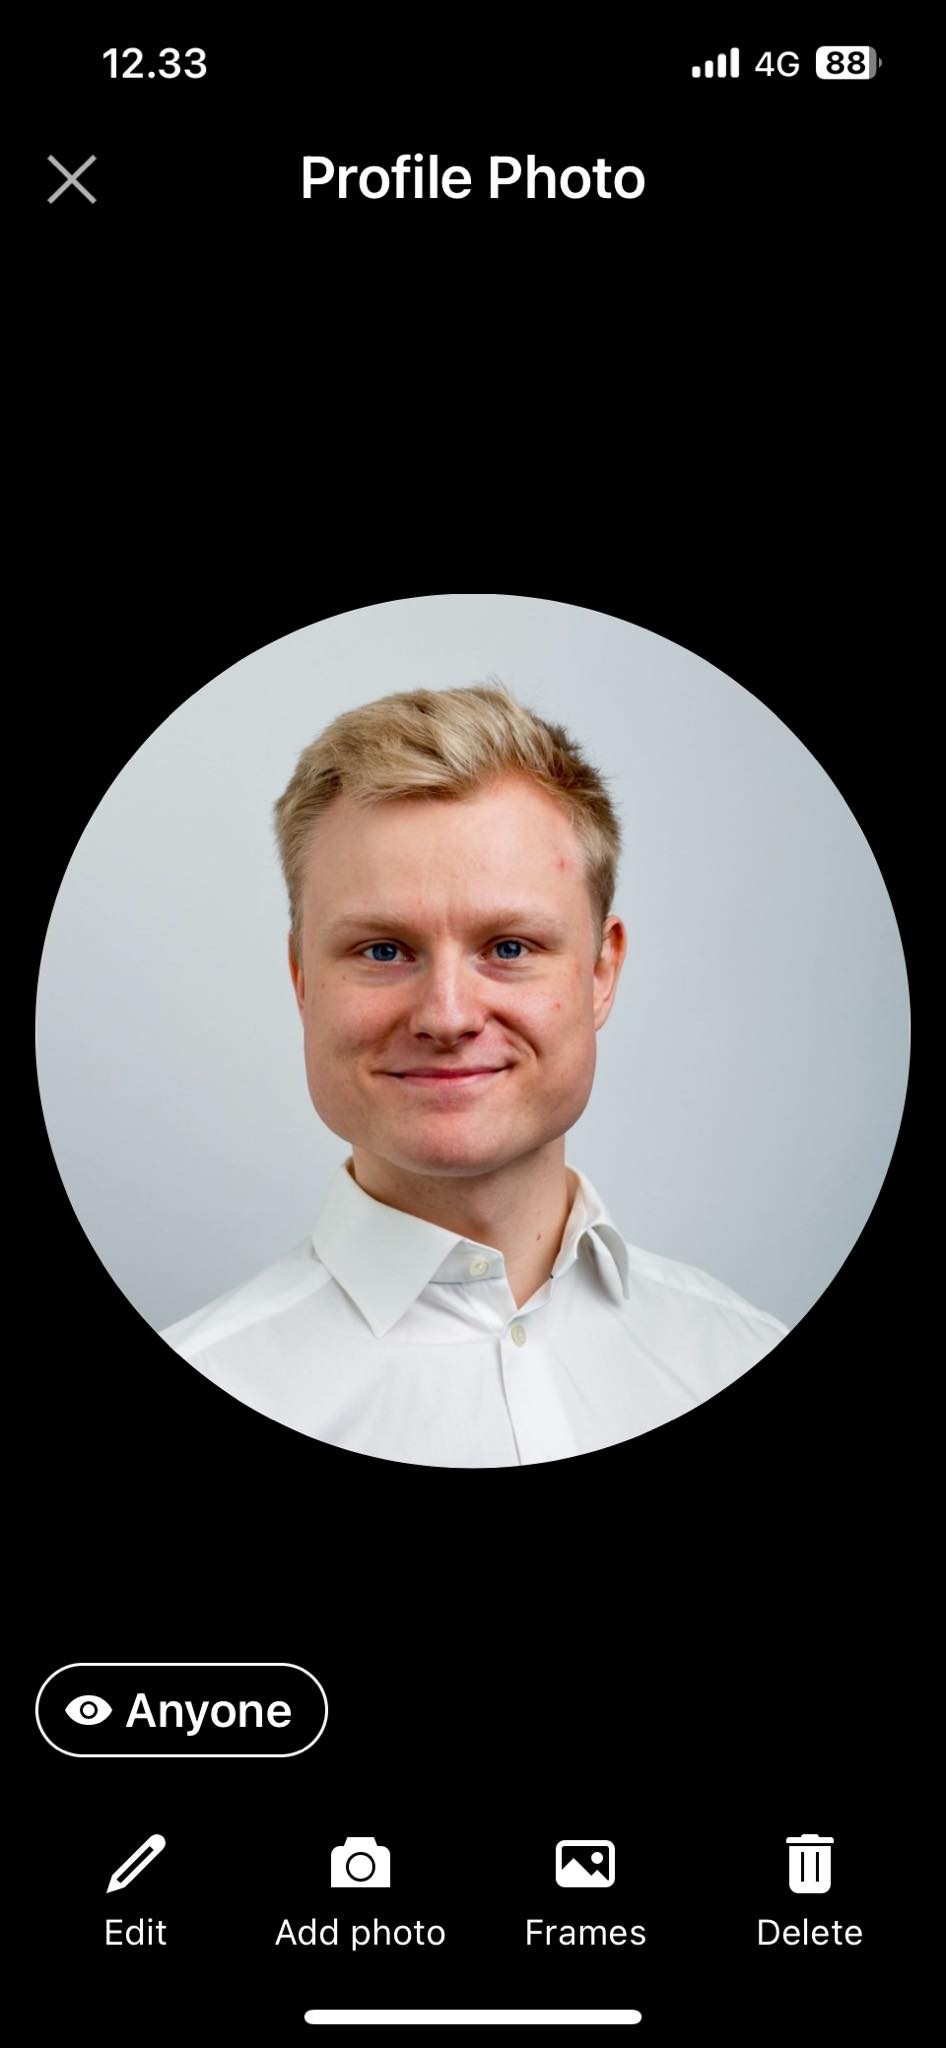
\includegraphics[width=9cm, trim={0mm, 200mm, 0mm, 200mm}, clip]{../../figures/picture_of_myself.jpg}

		
	\end{minipage}
	\begin{minipage}[c][3in][t]{0.48\linewidth}
			
		Contact Information:
		\begin{itemize}
			\item \textbf{Email}: cbrje@dtu.dk
			\item \textbf{Phone}: 0045 28 43 39 74
			\item  %\textbf{Website}: \href{http://www.yourwebsite.com}{www.yourwebsite.com}
		\end{itemize}
		
	\end{minipage}
}

\end{document}


% POSTER TEMPLATE AND GUIDANCE

% This document provides a guidance and set of minimum requirements for the research poster of the type made for the DTU Offshore Technology Conference. The aim is to improve the communication of the research to as wide an audience as possible.
% Size
% A0 format (841 x 1189 mm)
% Challenge
% In simple and concise terms state the following:
% •	What is the problem?
% •	Who is it a problem for?
% •	How big is the problem?

% Solution 
% •	How have the problem been solved? (if it is solved)
% •	What is the compelling unique solution?
% •	How will it be implemented?
% •	How is the problem going to be solved? (research hypothesis if not solved yet)

% Alternatives
% Why is this solution better than others?

% Connections and Context
% How does this research link to other projects?
% Is it based on a previous piece of work?
% How does this piece of work fit into the prototype as a whole?

% Other information can be useful to help the audience visualize the project. A time line of what has happened to bring you to this stage and what the proposed timeline is until completion. Again here the level of detail should be low and just show the major milestones.
% Of course, an acknowledgement of who the team is and what programme it is a part of is useful for some to put a face on the research.


